This section motivates the use of dynamic core fusion and its impact on performance and energy.
It also shows that loop optimizations have a significant performance impact when fusing cores.

\subsection{Dynamic Core Fusion}
\begin{figure}[t]
    \centering
    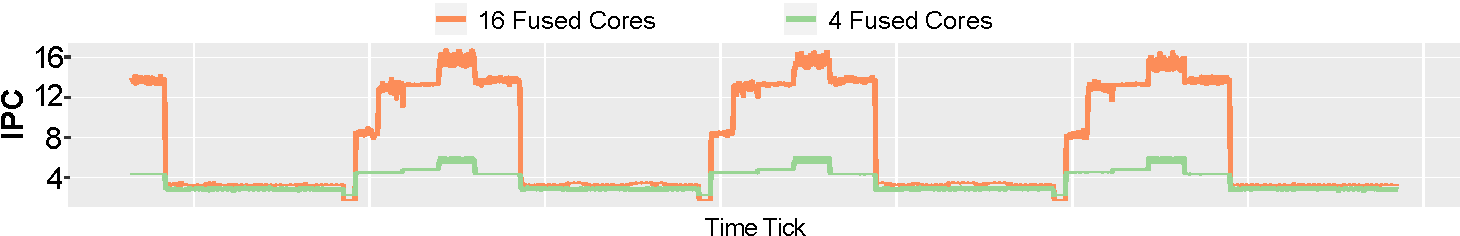
\includegraphics[width=\textwidth]{cases-paper/graphics/motivation/disp_opt_4_16_3.pdf}
    \caption{IPC of a typical benchmark (Disparity from SD-VBS) when executing on a fused 4 or 16 core processor.} 
    \label{fig:disp_ex}
	\vspace{1em}
\end{figure}
%\begin{figure}[t]
%    \centering
%    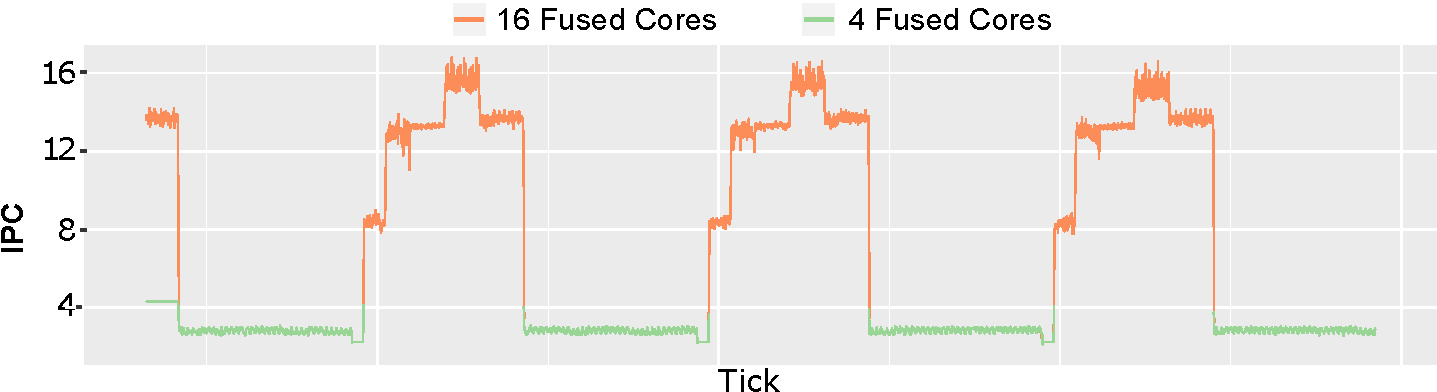
\includegraphics[width=\textwidth]{cases-paper/graphics/motivation/motiv3merge.pdf}
%    \caption{Example of ideal switching between 4 and 16 cores on a DMP for the Disparity benchmark.} 
%    \label{fig:ideal_switch}
%\vspace{2em}
%\end{figure}

Previous work in core fusion has focused on delivering performance improvements~\cite{ipek2007CoreFusion,kim2007tflex} and demonstrated how to predict static core fusion~\cite{micolet2016dmpstream}.
A static fusion fuses cores into a single logical core (LC) and executes a thread on this new core.
As evident from this prior work, fusion improves the performance of the program by maximizing speed.
However, as will be shown, static core compositions may not be the perfect match for all situations.

Figure~\ref{fig:disp_ex} plots the Instruction Per Cycle (IPC) performance variation over the execution of the \bm{Disparity} Benchmark from the San-Diego Vision Benchmark Suite (SD-VBS)~\cite{sdvbs} on core compositions of sizes 4 and 16 respectively.
IPC is a natural method of evaluating the performance of a core-composition as increasing the size of the composition should lead to a higher amount of instructions executing per cycle.
On 4 cores, the performance oscillates between an IPC of 2 and 6 depending on the phase while on 16 cores the IPC can be as high as 16.

In this Figure, the x-axis Tick represents a certain number of blocks that have been committed rather than being a measure of time in cycles.
This is why the high IPC phases for both core-compositions appear to last the same length of time even though the 16 core-composition executes the blocks faster.
In EDGE, a block is committed when it is no longer a speculative block and its memory and register operations have been committed back to memory or the register files.
The reason why number of blocks committed is used as a measurement of time is due to the fact that the number of blocks necessary to execute a program are independent of the size of a core-composition.

As can be seen in Figure~\ref{fig:disp_ex}, both the 4 and 16 core-compositions share the same IPC when it comes to the low IPC phase.
In a situation where the objective of the programmer is to maximise speed, without dynamic reconfiguration of the DMP, a static 16 core-composition will have to be used.
%Get actual energy estimations ot make this more clear
If the static 16 core composition is used, the DMP consumes 4 times as much energy to execute the low IPC phases compared to the 4 core-composition.
Thus, the static 16 core composition is considered energy inefficient during half the execution of the program.

On the other hand, if the DMP is reconfigured at runtime, the core-composition can switch to 4 cores when in the low-IPC phase to save on energy and switch to the 16 core composition when in the high IPC phase to maximise speedup.
In this situation, runtime reconfiguration allows to maximise speed whilst being energy efficient; a goal that cannot be achieved via static ahead of time configurations.

\subsection{Code Optimizations}
When cores are fused they execute blocks of instructions in parallel on each physical core in the logical core (LC).
In order to obtain the best results, large blocks must be generated as this leads to a higher IPC on the LC~\cite{micolet2016dmpstream}.
The optimizations applied include aggressive loop unrolling, inlining and replacing conditional statements with either software predication or architecture-level predication.
These optimizations are well known and do not require any structural modifications of the program.

\begin{figure}[t]
    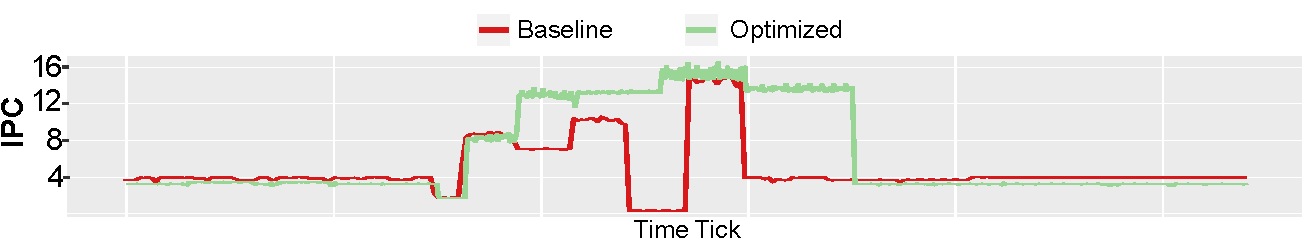
\includegraphics[width=\textwidth]{cases-paper/graphics/motivation/code_opt_3.pdf}
    \caption{Impact of loop transformations on fused cores for the Disparity benchmark.} 
    \label{fig:compmotiv}
\vspace{5mm}
\end{figure}
Figure~\ref{fig:compmotiv} illustrates the impact of applying loop transformations compared to a standard compiler not specifically tuned for an EDGE architecture.
As can be seen, the impact of these transformations can be large and are necessary to sustain a high IPC for a long enough period.
More details about the loop transformations are given in section~\ref{sec:opt} but this example illustrates the need for careful tuning of the compiler to achieve high performance on such an architecture.

\subsection{Summary}
This section has shown that programs exhibit phases with various amount of ILP available.
A dynamic multicore processor can take advantage of this property to fuse a large number of cores for the high-ILP phases and fuse a smaller number of cores when ILP drops to conserve energy.
The section also illustrated the importance of fine-tuned code transformations to achieve sustained performance and increase the potential for fusing cores.
The next section will study in more details the expected impact of fusion using an analytical model.

